\section{Projektplan}

\subsection{Projektstrukturplan}

\subsection{Meilensteinplan}
\subsubsection{Meilensteine}

\begin{itemize}
\item \textbf{M0} Ergebnis: Vorbereitungen sind getroffen, produktive Arbeit kann beginnen
\item \textbf{M1} Ergebnis: Hardware ist beschafft, Schnittstellen sind definiert
\item \textbf{M2} Ergebnis: Ausleihstation funktionst�chtig
\item \textbf{M3} Ergebnis: Lotus Notes Schnittstelle funktioniert
\item \textbf{M4} Ergebnis: Hardware ist eingebaut und getestet
\item \textbf{M5} Ergebnis: Funktionierendes Ausleihsystem, Produkt ist abgenommen
\end{itemize}

\subsubsection{Arbeitspakete}

\begin{itemize}
\item \textbf{AP0} Kickoff vorbereiten (eine Woche)
\item \textbf{AP1} Beschaffung und Test Hardware (eine Woche)
\item \textbf{AP2} Beschaffung M�bel (eine Woche)
\item \textbf{AP3} Definition der Schnittstelle Notes $\Leftrightarrow$ Ausleihstation (eine Woche)
\item \textbf{AP4} Testaufbau (inklusive Software) (zwei Wochen)
\item \textbf{AP5} Implementierung und Test der Schnittstelle Lotus Notes (vier Wochen)
\item \textbf{AP6} Einbau Kartenleser, T�rschloss, Kamera, Laser-Barcodescanner und Aufbau M�bel, Funktionstest (eine Woche)
\item \textbf{AP7} Abschlusstest und Abnahme (eine Woche)
\end{itemize}

\begin{figure}[h]
\begin{center}
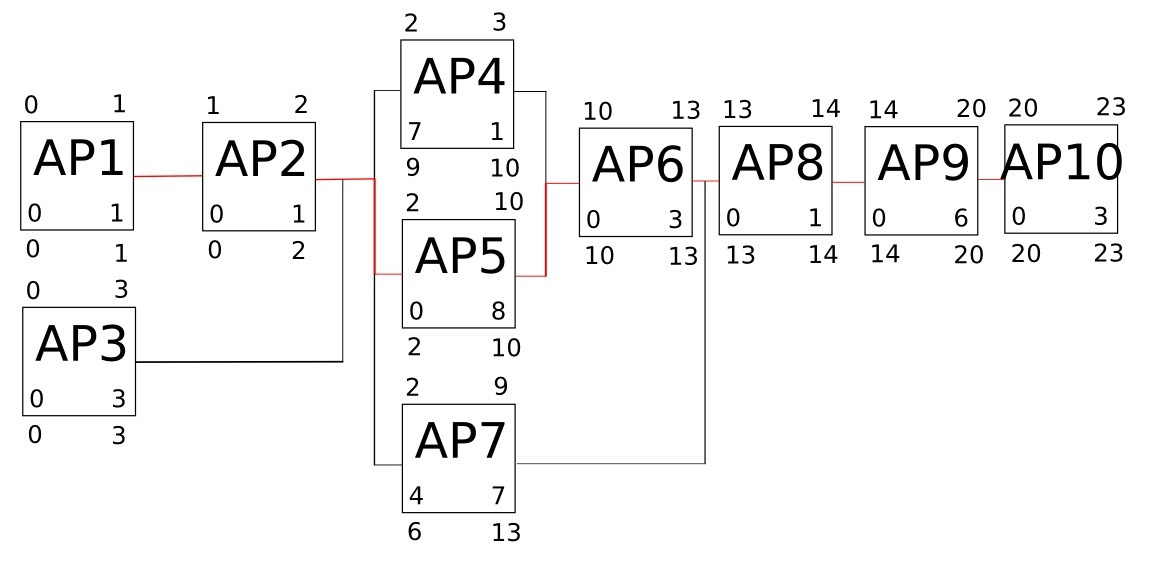
\includegraphics[width=0.8\textwidth]{abbildungen/netzplan.jpg}
\caption{Netzplan}
\end{center}
\end{figure}

\subsection{GANTT-Chart (Balkenplan)}

\begin{figure}[h]
\begin{center}
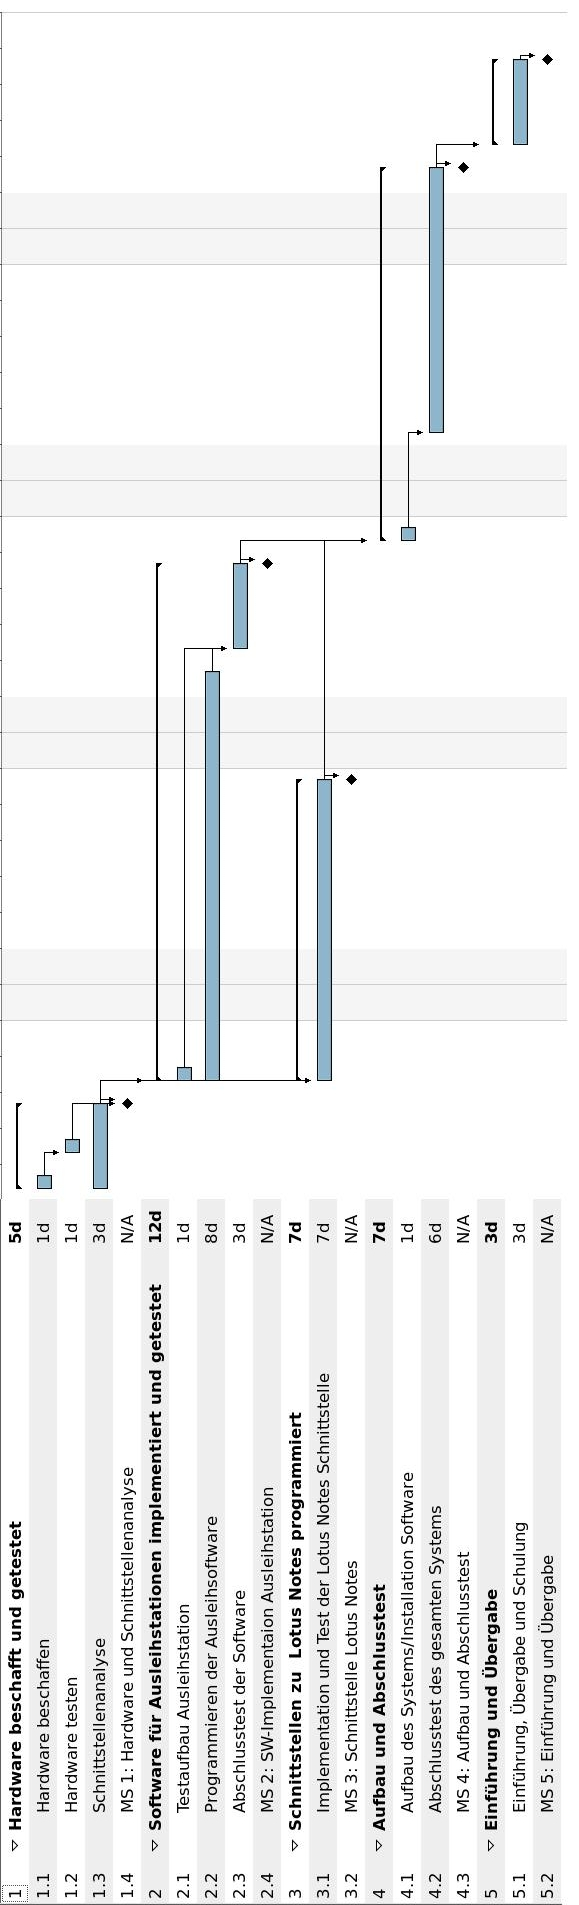
\includegraphics[width=0.8\textwidth]{abbildungen/gantt.jpg}
\caption{GANTT-Chart}
\end{center}
\end{figure}

\subsection{Kostens�tze}
Folgende Kostens�tze werden angenommen:
\begin{itemize}
\item 25 Euro f�r den einfachen Arbeiter
\item 35 Euro f�r den Denker
\end{itemize}

\subsection{Aufwands- und Kostensch�tzung}
\begin{table}[h]
\caption{Aufwands- und Kostensch�tzung}
\begin{tabular}[h]{|p{1cm}|p{4,8cm}|p{4,8cm}|p{2cm}|p{1,5cm}|}
\hline
\textsc{Nr} & \textsc{Aktivit�t} & \textsc{Rollen} & \textsc{Aufwand} & \textsc{Kosten}\\
\hline
1 & blub & blub & blub & 25\\
\hline
\end{tabular}
\end{table}

\subsection{Risikoplan}
\subsection{Werkzeuge}